\documentclass[14pt]{beamer}
\usepackage{fancyvrb}
\RecustomVerbatimCommand{\VerbatimInput}{VerbatimInput}{frame=single,
numbersep=1mm, numbers=left, formatcom=\color{orange}}
%\usepackage{kpfonts}
\usepackage[bitstream-charter]{mathdesign}


\mode<presentation>
{


\usetheme{Boadilla}
\useoutertheme{split}
\usecolortheme{albatross}

\setbeamertemplate{blocks}[rounded][shadow=false]
\setbeamertemplate{navigation symbols}{}



\setbeamercolor*{structure}{fg=green!75!black,bg=blue!70!white}
\setbeamercolor*{normal text}{fg=green!65!black,bg=blue!80!black}
\setbeamercolor{palette primary}{use={structure,normal text},fg=green,bg=structure.bg!75!black}
\setbeamercolor{palette secondary}{use={structure,normal text},fg=structure.fg,bg=structure.bg!60!black}
\setbeamercolor{palette tertiary}{use={structure,normal text},fg=structure.fg,bg=structure.bg!45!black}
\setbeamercolor{palette quaternary}{use={structure,normal text},fg=green,bg=structure.bg!75!black}
\setbeamercolor*{example text}{fg=green!65!black}
\setbeamercolor*{block body}{bg=structure.bg!90!black}
\setbeamercolor*{block body alerted}{bg=structure.bg!90!black}
\setbeamercolor*{block body example}{bg=structure.bg!90!black}
\setbeamercolor*{block title}{parent=structure,bg=structure.bg!75!black}
\setbeamercolor*{block title alerted}{use={structure,alerted text},fg=alerted text.fg!75!structure.fg,bg=structure.bg!75!black}
\setbeamercolor{item projected}{fg=white}
\setbeamercolor*{normal text}{fg=white!90!blue,bg=blue!70!black}
\setbeamercolor*{separation line}{}
\setbeamercolor*{fine separation line}{}
\setbeamercolor{alerted text}{fg=yellow}

}


\usepackage[italian]{babel}
\usepackage[utf8]{inputenc}
\usepackage{pgf}
\usepackage{verbatim}
\usepackage[ruled,vlined,linesnumbered]{algorithm2e}
\usepackage{amsfonts,eucal}

% \usepackage{euler}
% \usepackage[T1]{fontenc}


\author{Paola Bonizzoni \and Gianluca Della Vedova}
\title{The 1k genome project and data deluge}
\institute{Univ. Milano-Bicocca\\
%  \texttt{http://gianluca.dellavedova.org}%
}
\date{10 November 2014}
\pgfdeclareimage[height=1cm]{university-logo}{logounimib}
\logo{\pgfuseimage{university-logo}}

\DeclareMathOperator{\poly}{\text{poly}}
\DeclareMathOperator{\polylog}{\text{polylog}}


% If you wish to uncover everything in a step-wise fashion, uncomment
% the following command:
\beamerdefaultoverlayspecification{<+->}


\begin{document}

\begin{frame}
  \titlepage
\end{frame}

\begin{frame}\frametitle{Fact 1}
  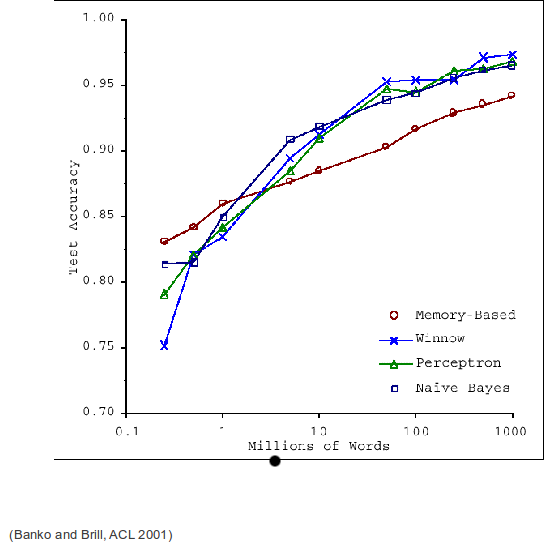
\includegraphics[width=5cm]{growing-data-1.png}
  \begin{itemize}
  \item
    Huge data are among us
  \end{itemize}
\end{frame}


\begin{frame}\frametitle{And more are coming}
  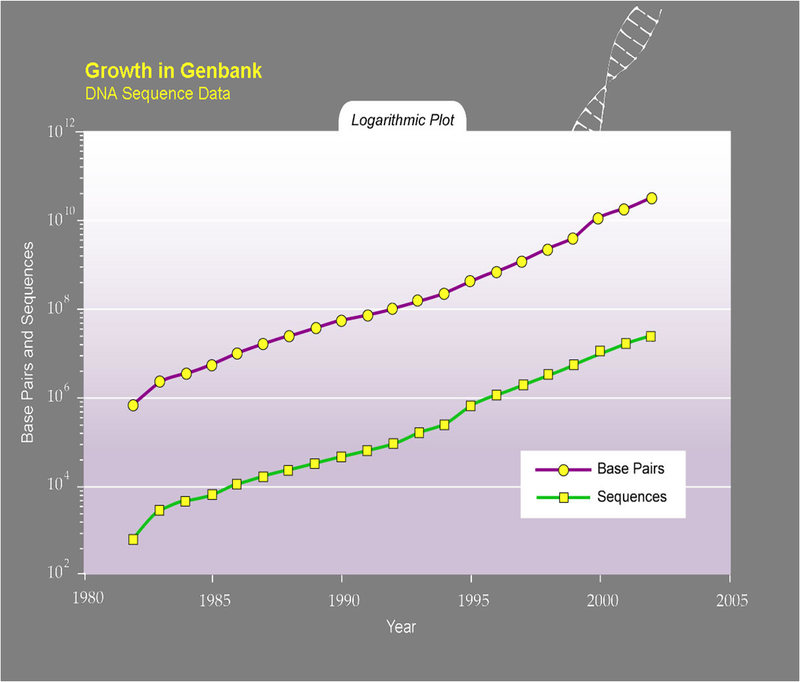
\includegraphics[width=6cm]{Kurzweil_DNA_Sequence_data_growth,_base_pairs_and_sequences_per_year.png}

  \small
  From 1982 to the present, the number of bases in GenBank has doubled
approximately every 18 months (\url{ftp://ftp.ncbi.nih.gov/genbank/gbrel.txt}).
\end{frame}

\begin{frame}\frametitle{Carlson Curve}
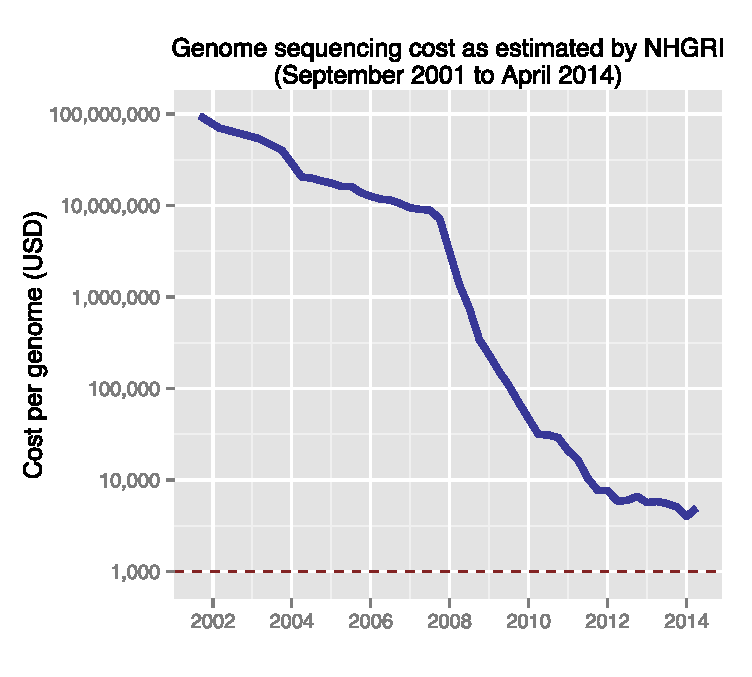
\includegraphics[width=6.7cm]{Historic_cost_of_sequencing_a_human_genome.pdf}

\small
DNA synthesis and sequencing productivity are both increasing at least as fast as Moore's Law.
[R.~Carlson.
The Pace and Proliferation of Biological Technologies, 2003]
\end{frame}



\begin{frame}\frametitle{Moore's Law}
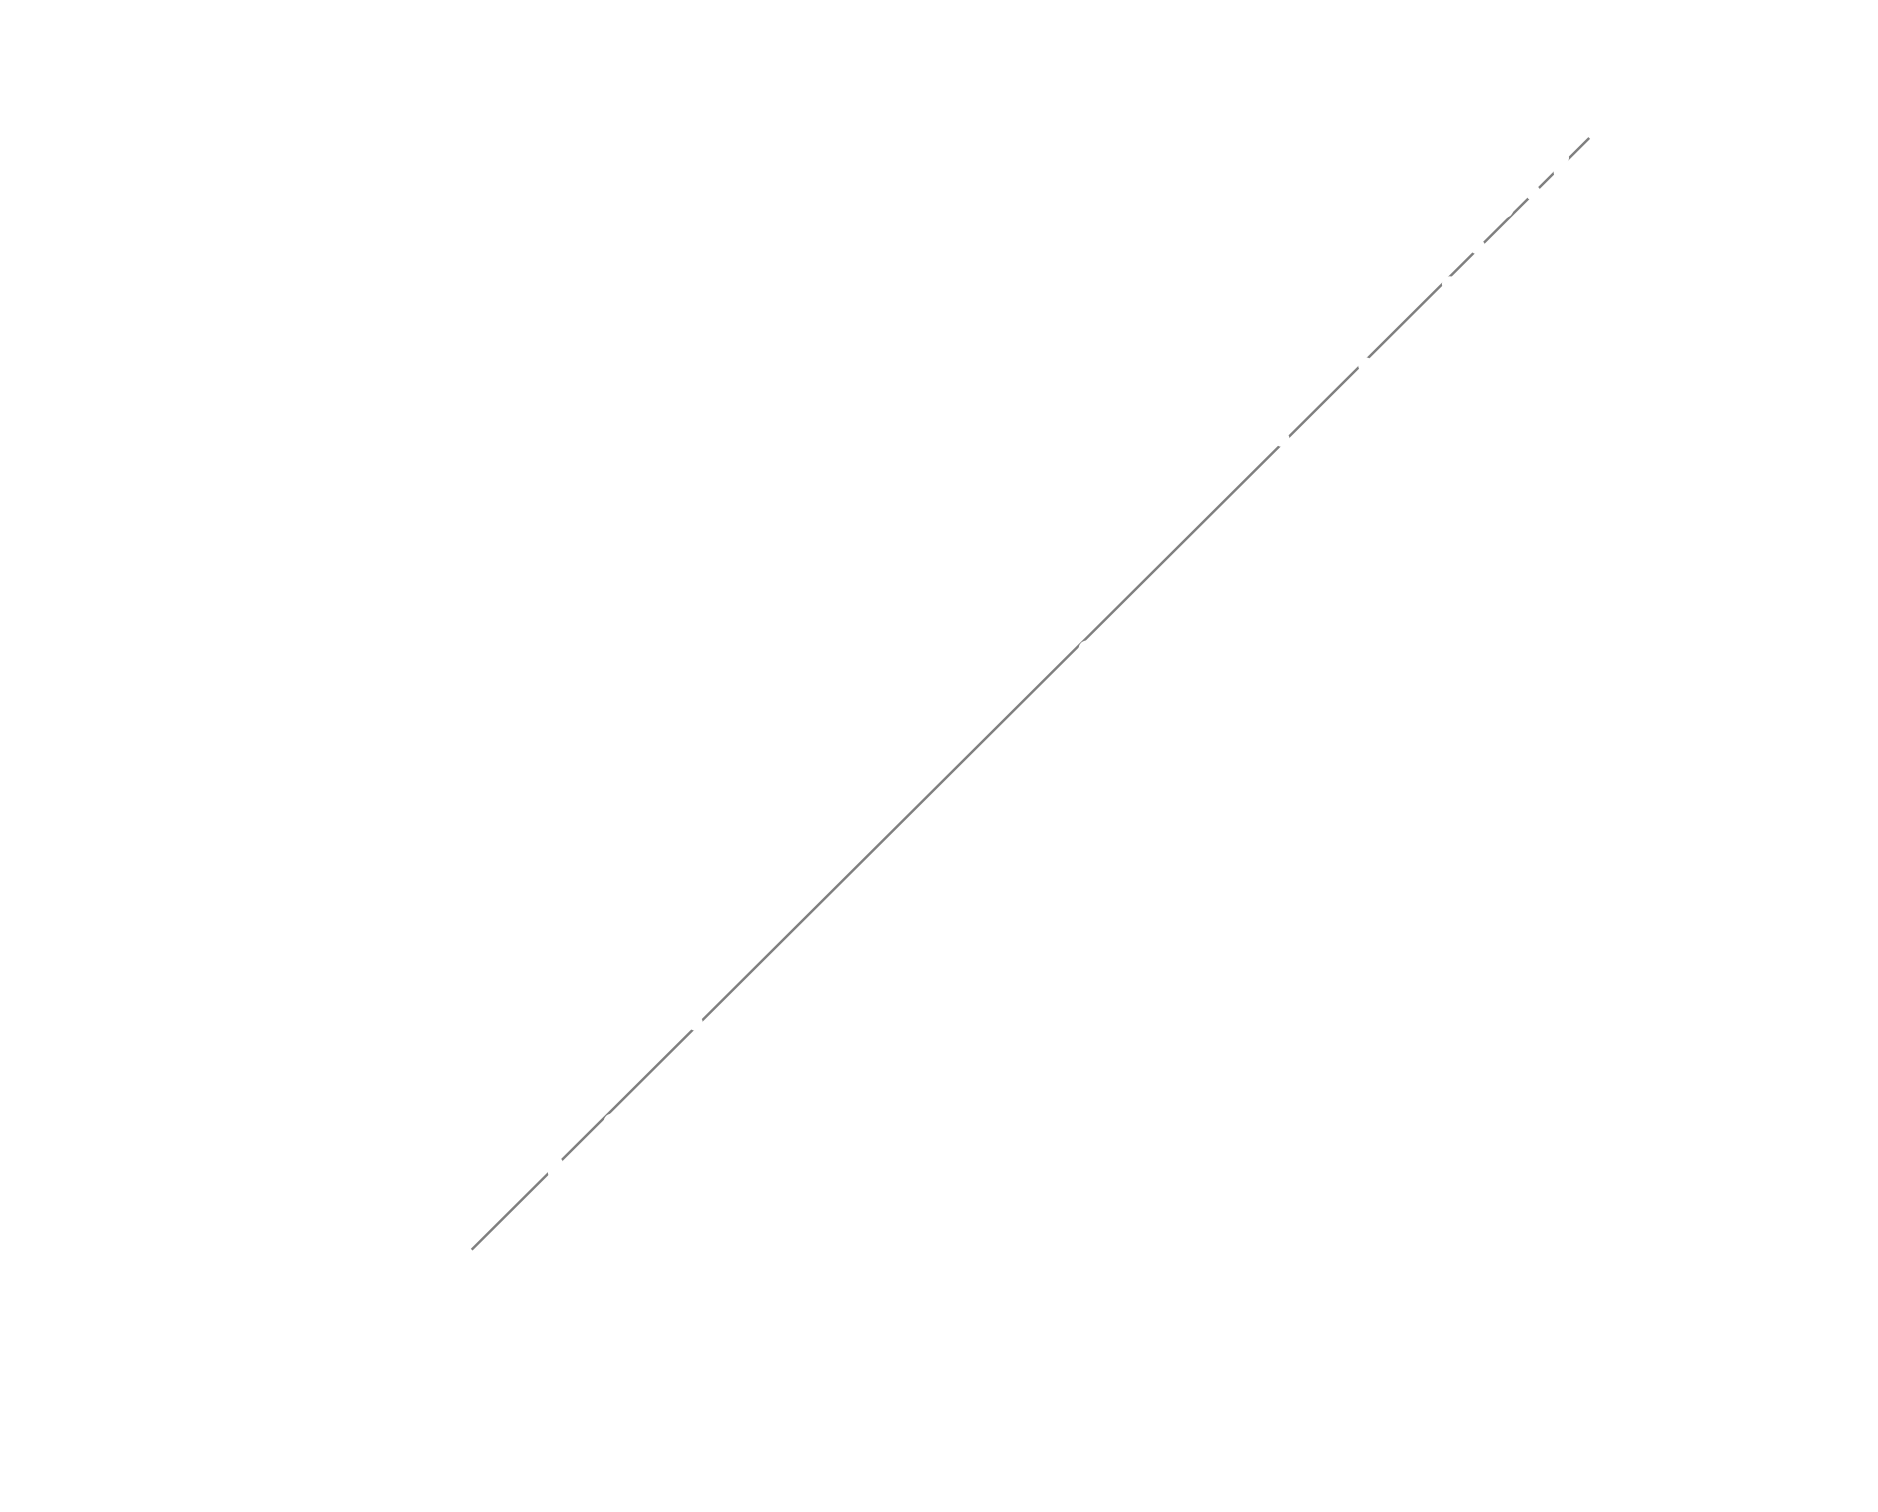
\includegraphics[width=9cm]{Moore_Law2.png}
\end{frame}


\begin{frame}\frametitle{Moore's Law is unfair}
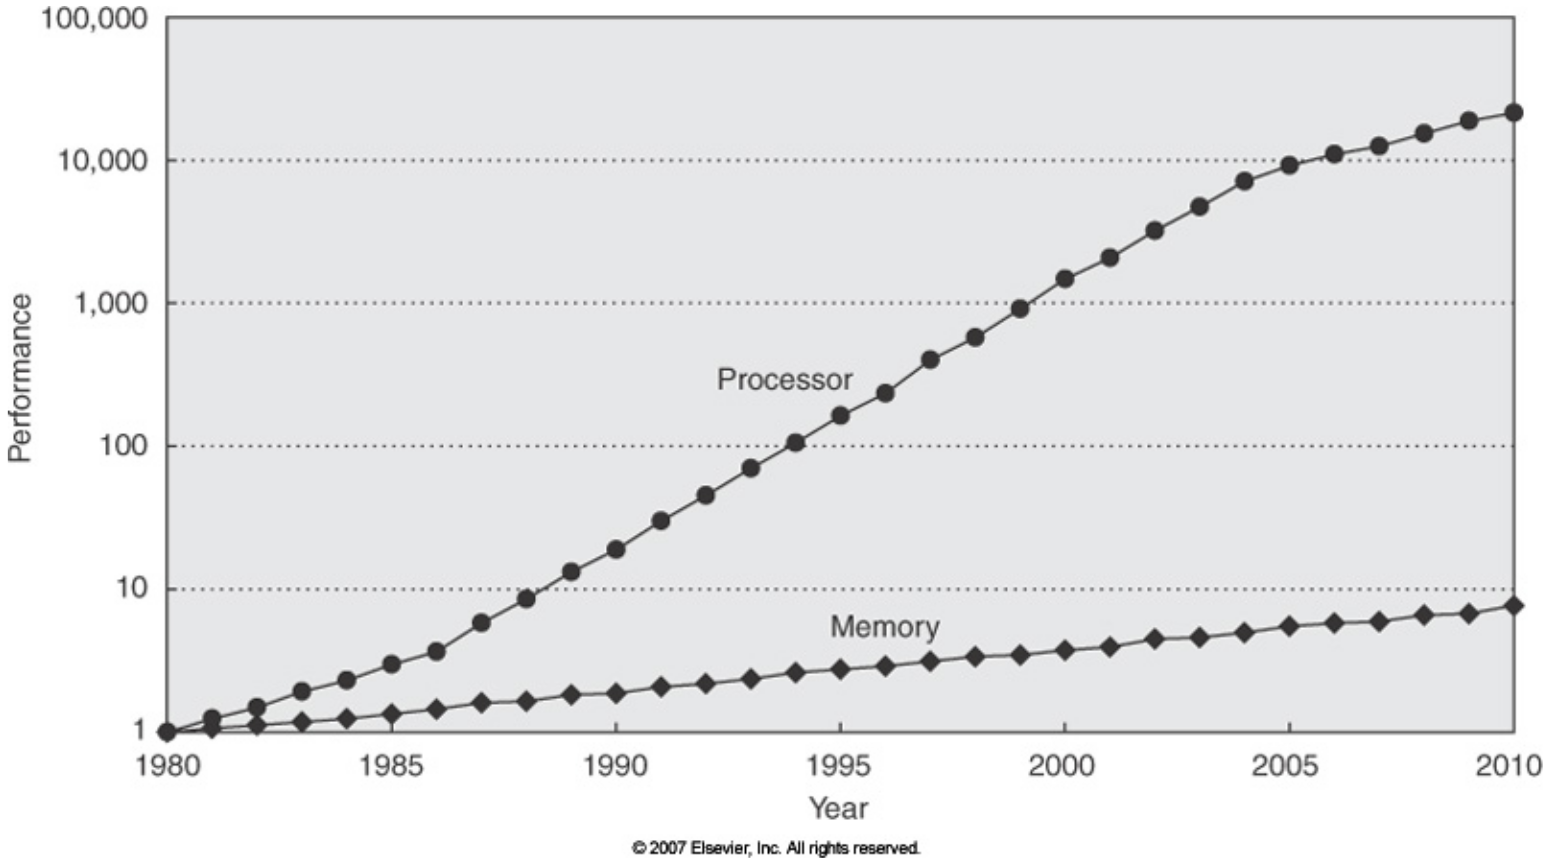
\includegraphics[width=11cm]{memory-cpu-gap.png}
\end{frame}

\begin{frame}\frametitle{Carlson Curve}
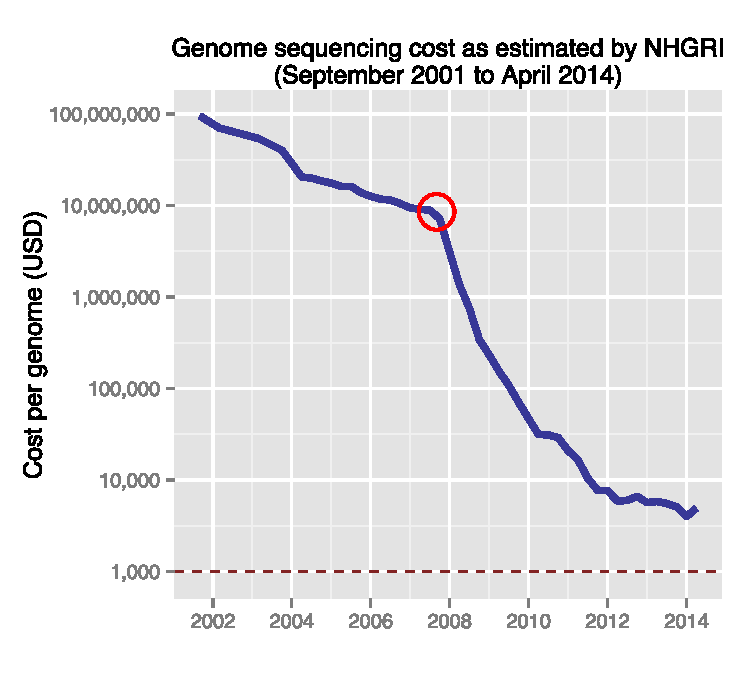
\includegraphics[width=6.7cm]{Historic_cost_of_sequencing_a_human_genome2.pdf}

\small
Next-Generation Sequencing Technologies
\end{frame}

\begin{frame}\frametitle{Different Technologies}


\small
\begin{tabular}{|p{8em}|p{3em}|p{2em}|p{2.2em}|p{1.9em}|p{1.8em}|p{2.3em}|}
\hline
Instrument&Primary Errors&Error Perc.&Read length&Run time&Gbp /run&cost /Gb\\
\hline
capillary (1st gen.)&subst.&0.1--1&650&2h&< 0.001&\$2.3M\\
\hline
454 FLX Titanium&indel&1&400&10h&0.4&\$15K\\
\hline
Illumina MiSeq v2&subst.&$\approx$0.1&50&5h&0.75&\$996\\
\hline
MiSeq v3&subst.&$\approx$0.1&150&20h&3.3&\$250\\
\hline
HiSeq 2500 rapid&subst.&$\approx$0.1&50&10h&15&\$90\\
\hline
HiSeq 2500 slow
&subst.&$\approx$0.1&250&6d&500&\$30\\
\hline
Ion Torrent Proton&Indel&$\approx$1&175&4h&12.25&\$82\\
\hline
Oxford Nanopore&dels&$\ge$4&3000&2h&0.09&\$1,100\\
\hline
PacBio RS&Indel&$\approx$13&9000&6h&0.9&\$1,000\\
\hline
\end{tabular}
\end{frame}


\begin{frame}\frametitle{Different Technologies}

\begin{figure}[h]
% \begin{subfigure}{0.45\textwidth}
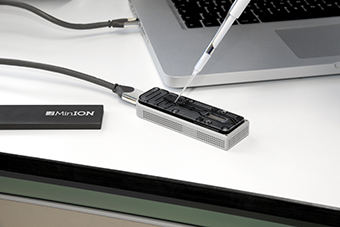
\includegraphics[width=0.45\textwidth]{4130_mini_ion_lab-copy}
\hfill
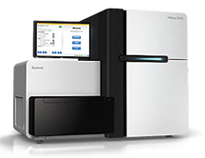
\includegraphics[width=0.45\textwidth]{illumna-hiseq20002}
\end{figure}
\end{frame}


% \begin{frame}\frametitle{Problem}
%   \begin{itemize}
%   \item
%     Input data too large for a single computer
%   \item
%     Don't fit into memory
%   \end{itemize}
% \end{frame}



\begin{frame}\frametitle{Dealing with NGS data}
  \begin{itemize}
  \item
    is a very difficult task!!!
    \begin{itemize}
    \item
      short fragments
    \item
      Different error distribution
    \item
      huge amount of data
    \end{itemize}
  \item
    Need of new algorithmic approaches and tools:
    \begin{itemize}
    \item
      time-space efficient processing (use of external memory)
    \item
      efficient data storage (data compression)
    \end{itemize}
  \end{itemize}
\end{frame}


\begin{frame}\frametitle{Credits}
\begin{itemize}
\item
``Historic cost of sequencing a human genome'' by Ben Moore. Licensed under Creative Commons Attribution-Share Alike 3.0 \tiny\url{https://commons.wikimedia.org/wiki/File:Historic_cost_of_sequencing_a_human_genome.svg}
\item
Moore's Law.
\tiny\url{https://en.wikipedia.org/wiki/File:Transistor_Count_and_Moore\%27s_Law_-_2011.svg}
\end{itemize}
\end{frame}

\end{document}

%%% Local Variables:
%%% mode: latex
%%% TeX-PDF-mode: t
%%% TeX-master: "bigdata-talk_video"
%%% buffer-file-coding-system: utf-8
%%% End:

